%%%%%%%%%%%%%%%%%%%%%%%%%%%%%%%%%%%%%%%%%%%%%%%%%%%%%%%%%%%%%%%%%%%%%%%%%%%%%%
% % % % % % %
%  Packages %
% % % % % % %

%---Base packages
\documentclass[a4paper,12pt,oneside]{report}	% document type (article, report, book)
\usepackage[utf8]{inputenc}			% encoding
\usepackage[T1]{fontenc}			% accent
\usepackage{lmodern}				% latin font
\usepackage{appendix}				% to be able to use appendices
\usepackage{tabularray}

%---Language(s)
\usepackage[english,frenchb]{babel}	% last language = typography by default
\addto\captionsfrench{				% to change the french names of...}
	\renewcommand{\appendixpagename}{Annexes}	% (default Appendices)
	\renewcommand{\appendixtocname}{Annexes}	% (default Appendices)
	\renewcommand{\tablename}{\textsc{Tableau}}	% (default \textsc{Table})
}

%---Page layout
%------> margins
	% 1st option -> geometry package
		%\usepackage[a4paper]{geometry}		% default parameters for A4
		%\usepackage[top=2in, bottom=1.5in, left=1in, right=1in]{geometry}
	% 2nd option -> a4wide package
		\usepackage{a4wide}		% A4 with smaller margins (the one I've chosen)
	% 3rd option -> fullpage package
		%\usepackage{fullpage}
%------> chapter style
	% 1st option -> fncychap package
		%\usepackage[style]{fncychap}		% style = Lenny, Bjornstrup, Sonny, Conny
	% 2nd option -> customized styles
		%
%------> cover page (UMONS template)
	\usepackage[fpms]{umons-coverpage}		% NEED "umons-coverpage.sty" file
	\umonsAuthor{Noms des auteurs : \\ Théau \textsc{Pauwels}}
	\umonsTitle{Synthèse - Intelligence numérique}
	\umonsSubtitle{Remise au propre et actualisation d'une synthèse}
	\umonsDocumentType{}
%	\umonsSupervisor{Sous la direction de : \\ Prof. T.\textsc{Dutoit} 
%                                            \\ Assistant H.\textsc{Bohy}}
	\umonsDate{Date: \\ 11 janvier 2025}

%---Numbering
\setcounter{secnumdepth}{2}			% numerotation depth (1=sec and all above)
\setcounter{tocdepth}{2}			% table of contents depth (1=sec and above)

%---Mathematics
\usepackage{amsmath}				% base package for mathematics
\usepackage{amsfonts}				% base package for mathematics
\usepackage{amssymb}				% base package for mathematics
%\usepackage{amsthm}				% theorem and proof environments
%\usepackage{cases}					% numcases environment
%\usepackage{mathrsfs}				% \mathscf command ('L' of Laplace-Transform,...)

%---Floating objects (images, tables,...)
\usepackage{float}					% better management of floating objects
\usepackage{array}					% better management of tables
\usepackage{graphicx}				% to include external images
\usepackage{wrapfig}
\graphicspath{ {./figures/} } 
%\usepackage{caption}				% /!\ has priority on "memoir" class
%\usepackage{subcaption}			% subfigure and subtable environments
%\usepackage{subfig}				% \subfloat command
%\usepackage{wrapfig}				% wrapfigure environment
%\usepackage[update]{epstopdf}		% to use '.eps' files with PDFLaTeX

%---Code including
\usepackage{listings}				% general package (can be tuned)
\usepackage{caption}
\newenvironment{code}{\captionsetup{type=listing}}{}
\usepackage[newfloat]{minted}
\usepackage{color}
%\usepackage[framed]{mcode}			% to include Matlab code
									% /!\ you need the "mcode.sty" file

%---Units from International System
\usepackage{siunitx}				% \SI{}{} command (units with good typography)
\DeclareSIUnit\baud{baud}			% definition of the "baud" unit
\DeclareSIUnit\bit{bit}				% definition of the "bit" unit

%---Drawing
\usepackage{tikz}					% useful package for drawing
\usepackage[european]{circuitikz} 	% to draw electrical circuits

%---Bibliography
\usepackage{url}					% to encore url
\usepackage[style=numeric-comp,backend=bibtex]{biblatex}
\usepackage{csquotes}				% inverted commas in references
\bibliography{bibli}				% your .bib file

%---"hyperref" package				% /!\ it must be the last package
\usepackage[hidelinks]{hyperref}	% clickable links (table of contents,...)
\hypersetup{
    colorlinks,
    citecolor=black,
    filecolor=black,
    linkcolor=black,
    urlcolor=black
}

% % % % % % %
% Document	%
% % % % % % %
%%%%%%%%%%%%%%%%%%%%%%%%%%%%%%%%%%%%%%%%%%%%%%%%%%%%%%%%%%%%%%%%%%%%%%%%%%%%%%
\hypersetup{ 	
pdfsubject = {Intelligence numérique},
pdftitle = {Remise au propre et actualisation d'une synthèse},
pdfauthor = {Théau Pauwels}
}
\begin{document}
\colorlet{bright-green}{green!45!white}
\colorlet{bright-red}{red!50!white}
\colorlet{bright-blue}{blue!30!white}
\colorlet{bright-orange}{orange!60!white}
% Ask for a regular cover page with full content and default picture
\umonsCoverPage 

% Table des matières
\tableofcontents
\newpage

\chapter{Codage de l'information}
    \section{Quantification}
        \subsection{Quantification uniforme}
            \colorbox{bright-blue}{Le pas de quantification reste constant.}\\
            $L$ : nombre de niveaux de quantification, $b$ : nombre de bits, $L = 2^b$\\\\
            $b\nearrow$ $\Rightarrow $ plus d'intervalles sur lesquels quantifier, ce qui augmente la qualité du signal \textbf{mais} augmente le débit \colorbox{bright-red}{(coût)}\\\\
            $b\searrow$ $\Rightarrow $ $\Delta \nearrow$, $\sigma_e ^2 \nearrow$ $\Rightarrow$ $RSB \searrow$. Pour les sons de faibles amplitudes, on aura une erreur relative \textbf{importante}. 
            \begin{center}
                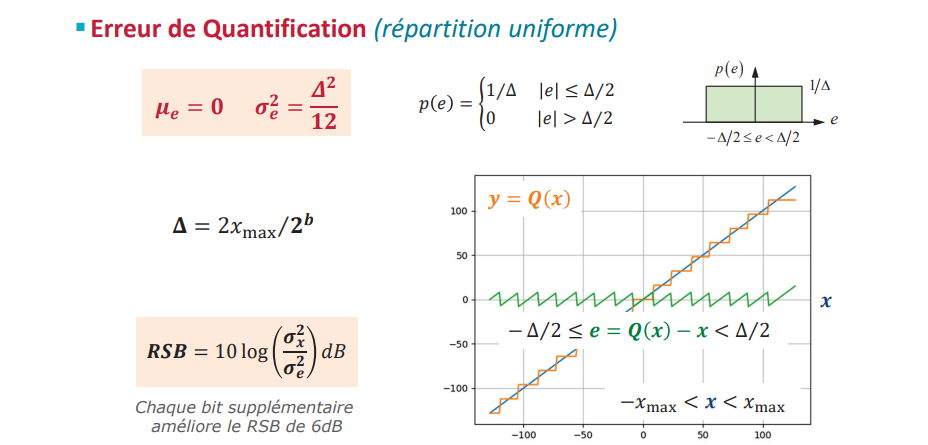
\includegraphics[width=13cm]{LaTeX/pictures/1.1.1_2.png}
                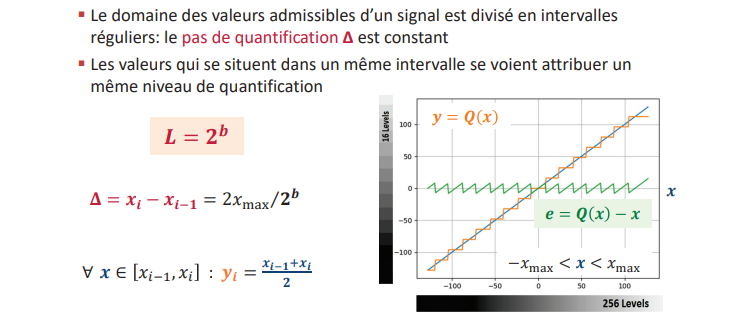
\includegraphics[width=13cm]{LaTeX/pictures/1.1.1_1.png}
            \end{center}
            
        \subsection{Quantification adaptative}
            \colorbox{bright-blue}{Le pas de quantification est proportionnel à l'écart-type du signal.}\\
            $\Delta = k.\sigma_x(\sigma)/2^b$\\
            $\Rightarrow$ proportionnel à l'énergie du signal $x$, cela résout le problème de la quantification uniforme qui ne quantifie pas bien les signaux de faibles amplitudes. Cette quantification adaptative permet de conserver un $RSB$ constant, mais elle implique aussi d'analyser le signal afin d'adapter le pas de quantification \colorbox{bright-red}{(coût)}
            
        \subsection*{Résumé quantification}
            En conclusion, si on est limité sur le nombre de bits, il est préférable d'opter pour quantification adaptative. Sinon, il est plus avantageux de pencher pour une quantification uniforme avec plus de bits.
\newpage

%%%%%%%%%%%%%%%%%%%%%%%%%%%%%%%%%%%%%%%%%%%%%%%%%%%%%%%%%%%%%%%%%%%%%%%%%%%%%%%%%%%%%%%%%%%%%%%%%

    \section{Codage de l'information}
        \subsection{Codage à longueur variable}
            \colorbox{bright-blue}{Association de symboles à un nombre de bits variable en fonction de leur probabilité.}\\
            Le principe est d'associer aux symboles de la source un nombre de bits variable. Afin d'économiser de l'espace (réduire le nombre de bits au total), les mots de codes les plus courts seront associés aux symboles les plus récurrents. Il s'agit donc d'un codage sans perte vu qu'aucune information n'est mise de côté durant cet encodage et que la source peut-être reconstituée intégralement. Cela requiert néanmoins que les symboles ne soient pas équitablement répartis afin qu'il soit efficient.\\\\
            Il est bon de rappeler qu'un évènement certain n'apporte pas d'information (on sait qu'il va se produire), et à l'inverse évènement improbable (changement soudain de couleur par exemple) est très important. On peut donc évaluer l'importance de l'évènement $x_i$ comme $I(x_i)=log_2(\frac{1}{P(X=x_i)})=-log_2(P_i)$.\\\\
            Le débit moyen $\bar{b}$ se calcule comme la somme du nombre de bits $n_i$ du symbole multiplié par la probabilité de ce symbole $P_i=P(X=n_i)$.\\
            De plus, à cause de sa nature statistique, le débit moyen est borné par l'entropie. 
            \begin{center}
                $\bar{b} = \sum_{i=1}^L P_i.n_i$ \\
                $H_Q = -\sum_{i=1}^L P_i.log_2(P_i)$, \quad \quad \quad $H_Q \le \bar{b} < H_Q + 1$
            \end{center}
            Pour savoir si le codage à débit variable est intéressant, il suffit de le comparer à un signal que l'on n'encoderait pas, c'est à dire le même nombre de bit que la source ; $\bar{b} < log_2(L)$ (pour rappel $L=2^b$).\\
            Il faut aussi faire attention que le codage prédictif propage les erreurs tout le long du message. En pratique il faut donc rajouter des symboles de synchronisation permettant de limiter la propagation en cas d'erreurs.
            \newpage
            \subsubsection{Code de Huffman}
                \begin{center}
                    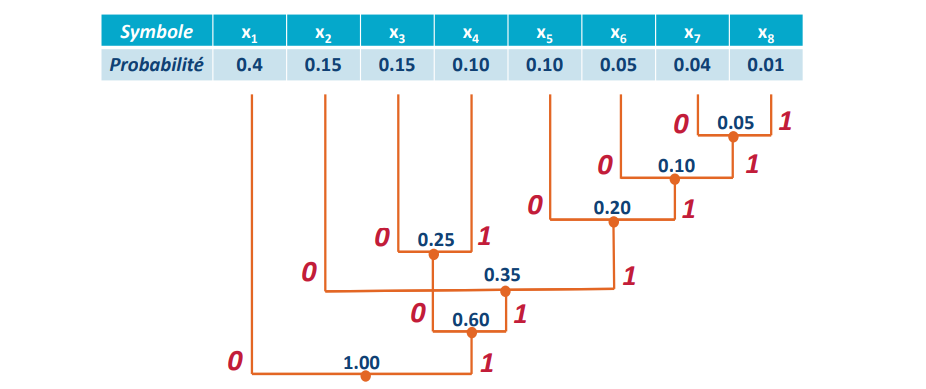
\includegraphics[width=13cm]{LaTeX/pictures/1.1.2_1.png}
                \end{center}
                Cependant le codage d'Huffman a un \colorbox{bright-red}{coût}: il faut calculer les probabilités de chaque symbole ainsi que la mémoire pour stocker le dictionnaire des valeurs. De plus, le code doit être transmis au décodeur pour reconstituer les symboles initiaux. Il est souvent moins coûteux de recalculer la table au décodeur.
            \subsection*{Résumé codage}
                \begin{center}
                    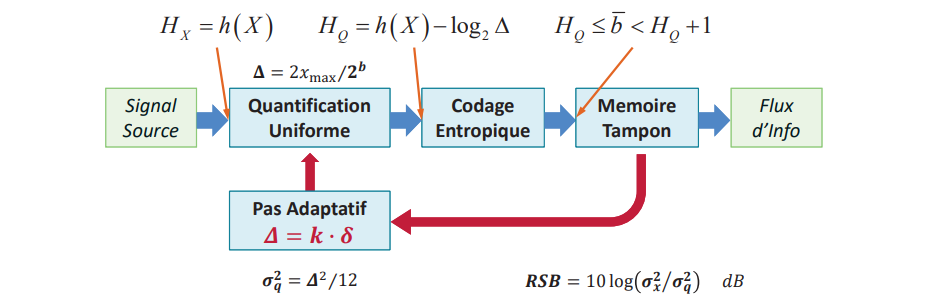
\includegraphics[width=13cm]{LaTeX/pictures/1.1.2_2.png}
                \end{center}
                Il y a plusieurs points d'attention dans ce schéma;
                \begin{itemize}
                    \item Si il s'agit d'une quantification adaptative, il faut faire attention de ne pas excéder la capacité mémoire de la mémoire tampon.
                    \item Si il s'agit d'une quantification uniforme, un grand pas implique une réduction de l'entropie (cool pour codage à longueur variable) donc on remplit moins vite le tampon, mais le $RSB$ se dégrade.
                \end{itemize}
                Il est préférable d'augmenter le bruit plutôt que de perdre de l'information, la quantification est donc à la fois uniforme et adaptative. Si les mots de code deviennent trop longs, on augmente la largeur des intervalles, ce qui réduit le nombre d'intervalles et donc le nombre de bits pour coder ces mots.\\\\
                Pour améliorer le codage entropique, on peut réduire l'entropie (réduire la redondance spatiale ou temporelle). En effet, le codage entropique considère les évènements statistiquement indépendants. Pour cela, on peut retravailler les données par exemple ;
                \begin{itemize}
                    \item Analyse en composantes principales
                    \item Transformée temps-fréquence
                    \item Prédiction
                    \item Codage par plage
                \end{itemize}

        \subsection{Codage prédictif}
            \colorbox{bright-blue}{Le codage prédictif permet d'estimer la valeur d'un échantillon (d'un symbole) sur base} \colorbox{bright-blue}{des précédents.}\\
            Par exemple pour une image, le lecteur va reconstituer de haut en bas et de gauche à droite. Au niveau de l'encodeur, on ne transmet que le signal d'erreur de prédiction. Ce modèle propose une bonne reproduction des zones uniformes (les zones de couleurs) mais une mauvaise des contours (changement brusque dans les couleurs).
            \begin{center}
                $x(k)=\sum_{i=1}^p a_i.x(k-i)+e(k) = \hat{x}(k) + e(k)$
            \end{center}
            Il faut donc trouver les $a_i$ qui minimisent $\sigma_e^2=E[(x-\hat{x})^2]<<\sigma_x^2$.\\
            Cependant il faut noter que les erreurs de quantification au décodeur s'accumule et font varier le signal reconstitué du signal initial. Il faut donc implémenter la reconstitution du signal dans la fonction qui calcule le signal d'erreur afin d'éviter un emballement de ces dites erreurs.
            \begin{center}
                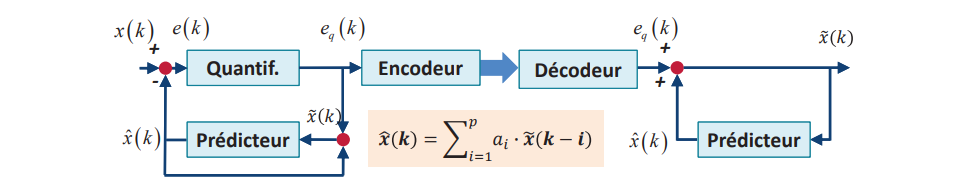
\includegraphics[width=13cm]{LaTeX/pictures/1.1.3_2.png}
            \end{center}
        \subsection{Codage hiérarchique (TP)}
            \colorbox{bright-blue}{Le but du codage hiérarchique est d'approximer l'image initiale avec un nombre très}\\ \colorbox{bright-blue}{réduit de valeurs.}\\
            On a une flexibilité des services de compression:
            \begin{itemize}
                \item Bas débit (accès rapide) pour un signal de faible qualité (approximation)
                \item Transmission progressive de données complémentaires selon la qualité requise
            \end{itemize}
            On peut notamment faire une décomposition en sous bande avec par exemple:
            \begin{itemize}
                \item Le filtrage miroir, un filtre passe bas (approximation) et un filtre passe haut (détails)
                \item Un sous échantillonnage (réduction de la résolution)
            \end{itemize}
\newpage
\chapter{Traitement de l'information}
    \section{Introduction}
        L'intelligence artificielle repose sur l'apprentissage (automatique ou supervisé) d'un système informatique. Utile quand il y a peu de théorie sur un sujet mais de grandes quantités de données. Le but de l'entrainment va être de soumettre l'IA à la donnée et de lui indiquer la sortie souhaitée ainsi qu'à quel point elle s'est trompée (fonction de coût).
%    \section{Concept général}
        %%%
    \section{Quantification vectorielle}
        Chaque observation est représentée par un vecteur contenant les caractéristiques observées (par exemple la température, la pression, ...). Il est possible de plotter ces données dans un graphe de même dimension que le vecteurs des caractéristiques. 

    \section{Clustering}
        Il est alors possible de classifier la donnée en l'associant à la référence la plus proche. ($N$ données, mais $K<N$ valeurs de références). La différence entre une quantification vectorielle et scalaire des données est la corrélation entre les variables.
        \begin{center}
            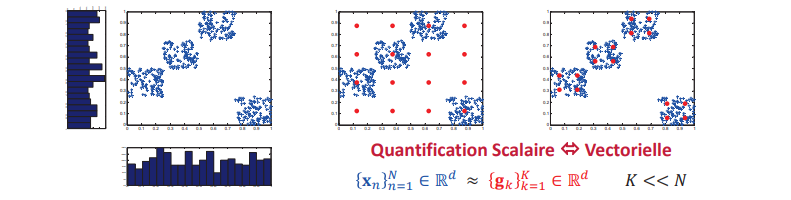
\includegraphics[width=13cm]{LaTeX/pictures/2.3_1.png}
        \end{center}
        
    \section{Algorithmes K-Means}
        Il s'agit d'une optimisation itérative où l'ordinateur va chercher à minimiser l'évolution du système (min. local dans la fonction de coût). L'avantage est qu'il peut déterminer lui même la classification et que le processus n'a pas besoin d'être supervisé.\\
        Un exemple de fonction de coût est la $MSE$ (mean squared error)
        \begin{center}
            $MSE= \frac{1}{N}\sum_{n=1}^N(\frac{1}{d} \sum_{i=1}^d[x_n(i)-g_k(i)]^2)<\epsilon_t$
        \end{center}
        Ou l'on itère jusqu'à ce que l'évolution de l'itération soit inférieure à ce taux
        \begin{center}
            $1<\frac{MSE(\tau-1)}{MSE(\tau)}<1+\epsilon_t$
            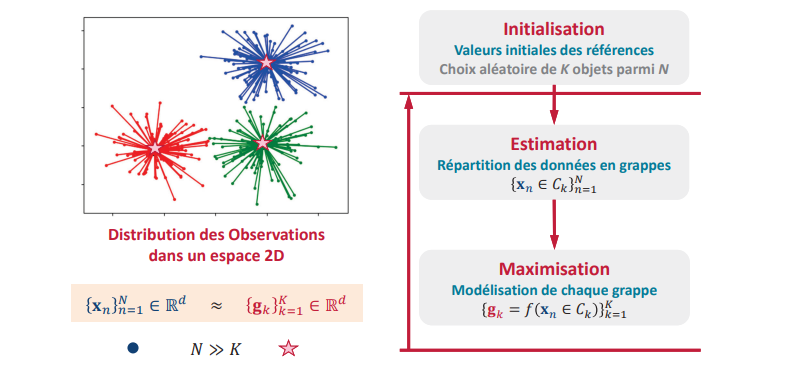
\includegraphics[width=13cm]{LaTeX/pictures/2.5_1.png}
        \end{center}
        
    \section{Approche hiérarchique}
        L'approche hiérarchique est l'approche des K-Means avec en plus la boucle de décision de l'ordinateur pour qu'il puisse rajouter de lui même des centroïdes.
        \begin{center}
            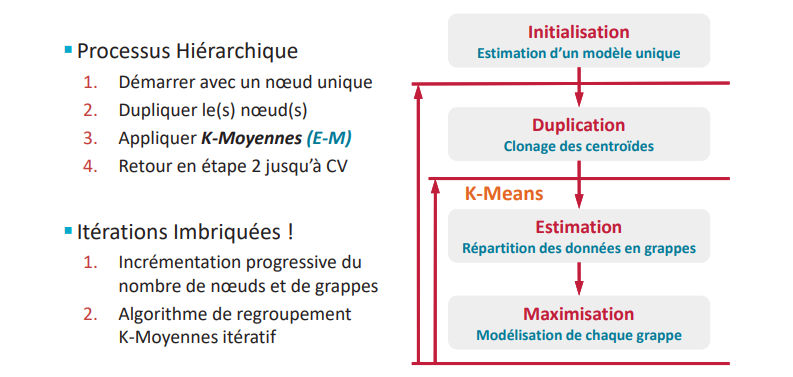
\includegraphics[width=13cm]{LaTeX/pictures/2.6_1.png}
        \end{center}
        C'est un processus beaucoup plus long et coûteux car il y $2^N$ centroïdes à présent
    \section*{Résumé}
        Les inconvénients de ces méthodes est que l'on ne se préoccupe pas des classes dans la création des clusters $\Rightarrow$ les clusters ne sont pas "purs", ils contiennent différentes classes de données. On attribue donc généralement la classe majoritaire aux clusters.
    \section{Analyse en composantes principales}
        Ici le but n'est pas de limiter le nombre de données mais de réduire le nombre de dimensions de représentation afin de réduire la taille de l'encodage de l'information.\\
        Pour cela on va définir une nouvelle base à partir de l'ancienne qui sera plus performante et représentera mieux les observations en réduisant possiblement les composantes.\\
        Il faut en préambule centrer les données (placer le centre des axes sur le centre de gravité des données) et normaliser ces dernières.
        \begin{center}
            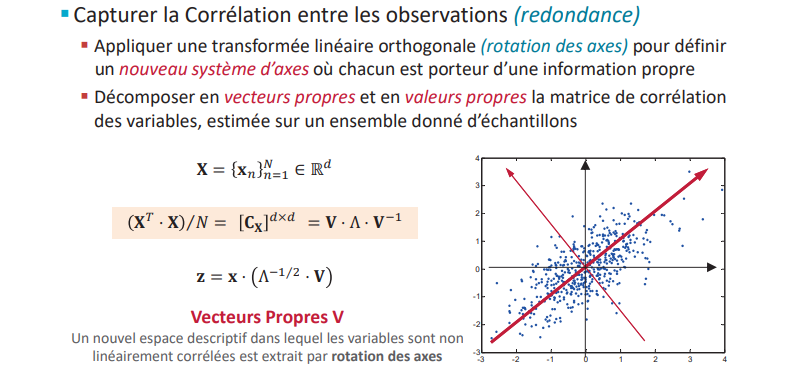
\includegraphics[width=13cm]{LaTeX/pictures/2.7_1.png}
        \end{center}
        Les nouveaux axes correspondent aux vecteurs propres $\vec{V_i} $ et les valeurs propres $\lambda_i$ associées représentent la dispersion des données autour de l'axe $i$ correspondant.
        \begin{center}
            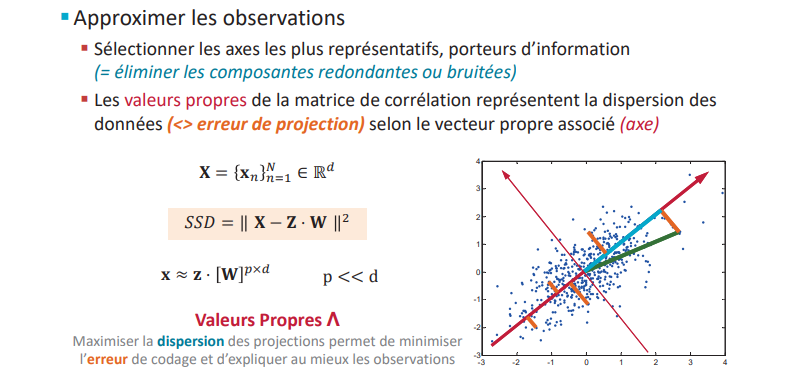
\includegraphics[width=13cm]{LaTeX/pictures/2.7_2.png}
        \end{center}
        En pratique, on va sélectionner les axes les plus significatifs, c'est à dire ceux avec la plus petite erreur de projection. \hyperlink{https://youtu.be/FgakZw6K1QQ?si=-eel9SYpv7jVf3en&t=303}{Cela correspond aux axes avec la plus grande dispersion*} et donc aux axes possédant les plus grandes valeurs propres.\\
        Il est bon de noter que le but de la PCA n'est pas de classer les données mais de les représenter. Vu qu'il n'y a pas de notions de classes, les composantes principales ne sont pas discriminantes.
\chapter{Introduction aux réseaux de neurones}
    \section{Neurone formel}
        Le neurone formel calcule la somme pondérée des entrées qu'il reçoit. Il compare ce résultat à une fonction d'activation non linéaire qui déterminera sa sortie. \\ 
        \colorbox{bright-blue}{La sortie d'un neurone formel est 1 ou 0}
        \begin{center}
            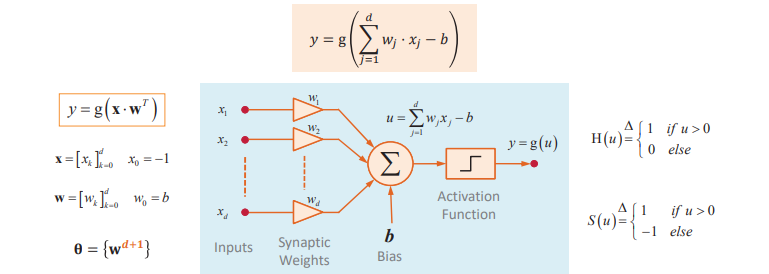
\includegraphics[width=13cm]{LaTeX/pictures/3.1.1_1.png}
        \end{center}
        Ici, la somme est comparée au seuil $b$ avant de passer dans la fonction d'excitation $g$. La fonction d'excitation sert à normaliser la valeur de sortie à 0 ou à 1 car la somme moins le biais $b$ peut avoir n'importe quelle valeur. A noter que les poids synaptiques $\omega_i$ sont ajustables. Ce sont eux qui influence l'importance des entrées sur le neurone.
    \section{Perceptron - S.L.P. (single layer perceptron)}
        \colorbox{bright-blue}{C'est un réseau de neurones possédant une seule couche (les entrées sont directement}\\ \colorbox{bright-blue}{reliées aux neurones de sorties).}
        Il s'agit d'un système discriminant car on assignera 1 neurone de sortie par classe d'objet.\\
        Pour l'apprentissage supervisé, on présente un objet à l'entrée du réseau de neurones. Ce dernier va faire une prédiction, il faut alors de lui présenter la classe attendue (notion de coût) afin qu'il ajuste si nécessaire ses paramètres. Le modèle devra alors minimiser l'écart entre les sorties réelles et les classes cibles.
        \subsection*{Avantages}
            C'est un modèle simple à entraîner.
        \subsection*{Inconvénients}
            Il ne marche que pour des problèmes linéaires et il peut être trop discriminant.
        \subsection*{Apprentissage}
            Pour l'apprentissage, on va utiliser la méthode du gradient (on cherche un minimum local, et si possible le global). Pour cela, on a besoin d'une fonction d'erreurs pour comparer la sortie du perceptron à la sortie attendue. Nous utilisons le critère des moindres carrés :
            \begin{center}
                $E = \sum_{n=1}^N \sum_{i=1}^m (\Phi_i(i_n)-t_{n_i})^2$ 
            \end{center}
            Avec $\Phi_i(i_n)$ la sortie obtenue grâce à la fonction d'activation. Fonction que l'on choisit continue que l'on pourra dériver : par exemple la sigmoïde $S(x) = \frac{1}{1+e^{-x}}$\\
            Pour minimiser les poids de chaque neurone, on va utiliser la méthode du gradient ;
            \begin{center}
                $\omega(\tau+1)=\omega(\tau) - \alpha . \frac{\partial E}{\partial \omega}(\tau)$
            \end{center}
            Avec $\alpha$ le taux de convergence, il s'agit d'un compromis entre vitesse de convergence, et ne pas dépasser le minimum que l'on souhaite atteindre. C'est une méthode assez longue mais qui donne de très bons résultats. 
        
    \section{M.L.P. (Multi-layer perceptron}
        Le principe de la MLP est le même que la SLP sauf que l'on va venir placer plusieurs couche en cascade les unes des autres (c'est toujours la dernière qui prend la décision), il s'agit toujours d'un modèle discriminant. Cela permet d'augmenter la capacité du modèle au détriment d'une augmentation aussi de sa complexité.\\
        L'apprentissage du MLP se fait en 2 étapes ;
        \subsection*{Propagation}
            On présente une partie des échantillons au modèle en indiquant pour chacun la sortie souhaitée. En fonction de la sortie réelle du réseau, on calcule sa fonction de coût (à quel point il s'est trompé) 
        \subsection*{Retropropagation}
            Chaque neurone effectue un retour en arrière via la retropropagation pour minimiser l'erreur commise (les poids vont être ajustés)\\\\
        En réitérant ces étpaes sur d'autres partie des échantillons, il est possible d'entraîner le modèle jusqu'à ce qu'il n'évolue plus de manière significative. Il est possible de réduire le nombre d'itérations en effectuant d'autres traitements préalables comme une quantification vectorielle.
    \section{Estimation du gradient}
        L'estimation du gradient peut se faire de deux manières différentes :
        \begin{itemize}
            \item L'entraînement stochastique; calcul du gradient pour chaque point de donnée et recalcule de tous les poids. Très long et fastidieux, et les corrections "aléatoires" (dans un sens, puis dans l'autre). \colorbox{bright-red}{Énormément d'itérations et gros temps de calcul}
            \item Batch training; On présente tous les caractères et on accumule tous les gradients d'erreurs. On ne corrige les poids qu'après avoir présenté toutes les données. (On fait une moyennes des différents gradients afin de trouver la direction minimisant l'erreur). \colorbox{bright-red}{On ne fait qu'une seule correction des poids pour l’ensemble des caractères} mais \colorbox{bright-green}{plus rapide et moins coûteux en calcul.}
        \end{itemize}
        La méthode la plus efficace est donc un compromis, on va prendre des paquets d'échantillons (que l'on espère représentatifs pour pouvoir nous donner une bonne approximation du gradient total) et on va réévaluer les poids plusieurs fois sur l'ensemble des données d'entraînement.\\\\
        L'effet mémoire permet d'adoucir l'estimation du gradient global et de rendre la démarche moins "aléatoire". \\
        Les paramètres d'apprentissage $\alpha$ et $\beta$ sont fixés par l'utilisateur et doivent être optimisés. 
        \begin{center}
            $\Delta \omega(k) = -\alpha. \nabla E(k)$            
        \end{center}
        En cas de faible pente, il faut un $\alpha$ suffisamment petit pour ne pas osciller autour du point d'équilibre. Mais un faible $\alpha$ implique une faible correction et donc un temps de convergence plus long. Pour faire face à cela, il est possible d'utiliser un taux d'apprentissage adaptatif $\alpha(\tau)$ pour accélérer la convergence.\\
        Si d'une itération à une autre, l'erreur diminue, alors on sait que l'on est dans la bonne direction donc on peut augmenter $\alpha$. Si l'erreur augmente mais de moins de $5\%$, on garde $\alpha$ et on continue, si l'erreur augmente de plus de $5\%$, alors on revient en arrière pour diminuer $\alpha$. \colorbox{bright-green}{Faible surcharge de calcul et bonne efficacité pour une seule couche cachée.}\\
        L'approximation des méthodes de minimisation du $2^{nd}$ sont aussi efficace, mais la surcharge de calcul est de mémoire est significative (mais parfois acceptable). \colorbox{bright-green}{Très bonne efficacité} \colorbox{bright-green}{pour les MLP avec plusieurs couches cachées.}\\
        Pour générer un gradient plus significatif, il est possible d'utiliser des fonctions d'activations alternatives. Par exemple la \textcolor{red}{sigmoïde} sature au niveau des extrémité ($\Rightarrow$ \textcolor{blue}{dérivée} en cloche). Dans les états incertains il y aura donc une grande variation tandis que dans les états certains le gradient sera très faible. \\
        \begin{center}
            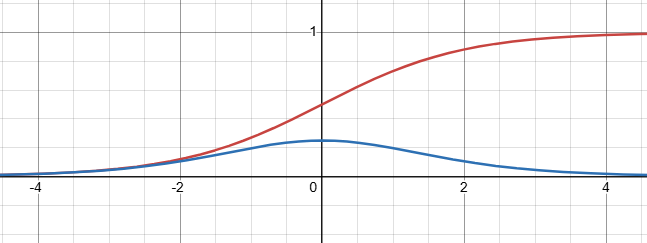
\includegraphics[width=13cm]{LaTeX/pictures/3.4_1.png}
        \end{center}
        A noter que cette minimisation pourrait mener à se retrouver dans un minima local plutôt que global, risque d'autant plus grand que le nombre de couches cachées augmente.
        \subsection*{Avantages}
            \begin{itemize}
                \item Apprentissage discriminant
                \item Permet de gérer des problèmes plus complexes
                \item Le réseau est capable d'approximer n'importe quelle opération entre l'espace d'entrée et l'espace de sortie
                \item En théorie une seule couche cachée est suffisante
                \item Les sorties d'une réseau de neurones entraînés pour la classification sont une bonne approximation des probabilités à posteriori
                \item Les MLP sont plus précis que les SLP
            \end{itemize}
        \subsection*{Inconvénients}
            \begin{itemize}
                \item Il n'existe pas de règles pour déterminer le nombre optimal de couches cachées, il faut trouver sur base d'expérimentation
                \item Les unités cachées génère des moments d'ordre élevés à partir des entrées. On ne retiendra que les éléments pertinents, il faut donc filtrer les moments inutiles
                \item Risque structurel élevés dû aux hypothèses prises
                \item Apprentissage itératif et \colorbox{bright-red}{chronophage}
                \item C'est un modèle en boite noire, nous ne savons pas exactement comment le modèle raisonne
                \item Risque de tomber dans un minimum local
                \item Risque de surapprentissage. Pour le limiter, il faut faire de la validation croisée en conservant une partie des données pour la validation. Il apparait quand on effectue trop d'itération (le modèle commence à modéliser le bruit autour des objets)
            \end{itemize}
    \section{Réseaux de neurones profonds}
        \colorbox{bright-blue}{Le but est d'automatiser l'étape d'extraction des caractéristiques.}\\
        Pour ce faire, on va employer un apprentissage discriminant afin d'entraîner un modèle d'extraction de telle manière à ce que les couches cachées soient responsables de la quantification vectorielle et du clustering, et que la couche de sortie soit responsable de la classification. 
        \subsection*{Avantages}
            \begin{itemize}
                \item Génère des fonctiones discriminantes non linéaires ($\equiv$ MLP)
                \item Apprentissage plus rapide mais sans optimisation globale
            \end{itemize}
        \subsection*{Inconvénients}
            \begin{itemize}
                \item Temps d'entraînement plus élevé que MLP
            \end{itemize}
    \section{Réseaux de neurones convolutionnels - C.N.N. (convolutional neural network)}
        Pour l'extraction des caractéristique, on va scinder le problème complexe en différents niveaux. Les concepts les plus simples sont fusionnés pour en construire des plus abstraits pour la machine (exemple reconnaissance de chiffres; reconnaitre des bouts de lignes [pas de sens pour nous], reconnaîtres des formes simples [cercles, barre horizontale/verticale,...], reconnaitres des chiffres).\\\\
        Les réseaux de neurones convolutionnels fusionnent l'extraction (couches de convolution pour l'extraction des caractéristiques) et la classification (par un MLP).
        \subsection*{Les couches de convolutions}
            Sur une carte (sous région de l'observation), chaque neurone prend en compte une partie des entrées (structure locale). Les neurones d'un même carte partagent les mêmes poids (il y a une invariance à la translation) \colorbox{bright-blue}{Les neurones partageant les mêmes poids extraient des}\\ \colorbox{bright-blue}{caractéristiques similaires à des endroits différents.} Il faudrait différentes cartes pour extraire différentes caractéristiques.\\\\
            Afin de diminuer la dimension (et la charge de calcul) et pour extraire le plus important de la zone, on va introduire des couches de sous-échantillonage.
            \newpage
            On peut refaire une convolution (convolutions multicouches) pour augmenter le niveau d'abstraction et extraire des caractéristiques de plus en plus complexes et recherchées (traitement profond).
            \begin{center}
                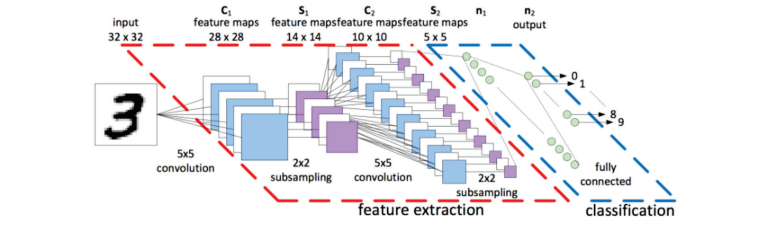
\includegraphics[width=13cm]{LaTeX/pictures/3.6_1.png}
            \end{center}
            Les CNN extraient des caractéristiques discriminantes avec un risque controlés. L'extraction des caractéristiques est discriminante et l'apprentissage subitune optimisation globale. Lalgorithme est développé sur base d'une retropropagation dédiée.\\
            Le risque structurel est sous contrôle: l'apprentissage est facilité par le nombre réduit de paramètres libres (neurones pas tous interconnectés, poids partagés et sous échantillonage $\Rightarrow$ réduction du nombre de poids).\\
            \colorbox{bright-blue}{L'augmentation des données améliore les capacités de généralisation.}
            
\chapter{Systèmes dynamiques}
    \colorbox{bright-red}{Note aux prochains}, aller en cours et faites une vraie synthèse de ce chapitre. ChatGPT va pas nous carry de ouf la dessus.
    \section{Introduction}
        \colorbox{bright-blue}{Les systèmes dynamiques visent à estimer une distance ou une probabilité.}
        Ils jouent un rôle fondamental dans l’étude et l’analyse des données temporelles, c’est-à-dire des séries d’observations collectées au fil du temps. Ces systèmes permettent de modéliser, de comprendre et de prédire le comportement de phénomènes évoluant dans le temps, qu’ils soient naturels, mécaniques ou numériques.\\\\
        Un système dynamique se définit comme un modèle ou un ensemble de règles décrivant l'évolution d’un état en fonction du temps. Il s'agit d'un outil puissant utilisé dans de nombreux domaines, comme la reconnaissance de formes, le traitement de signaux, ou encore la surveillance de systèmes industriels. Contrairement à une analyse statique, les systèmes dynamiques s’intéressent à l'évolution des données, permettant ainsi de capturer des relations complexes entre les observations.\\\\
        Les objectifs de cette introduction sont;
        \begin{itemize}
            \item \textbf{Comprendre les séries temporelles} : Leur nature, leurs propriétés et les défis qu’elles posent (longueur variable, bruit, etc.).
            \item \textbf{Maîtriser les outils d’analyse dynamique} : Par exemple, l’alignement dynamique des séries (Dynamic Time Warping - DTW) et les modèles probabilistes comme les modèles de Markov cachés (HMM).
            \item \textbf{Appliquer ces outils à des cas concrets} : Reconnaissance de motifs, comparaison de séquences, prédiction de comportements.
        \end{itemize}
        L’intelligence numérique repose sur la capacité à extraire des informations pertinentes à partir de données complexes. Les systèmes dynamiques apportent une solution unique pour traiter des séquences de données non stationnaires, en intégrant des modèles mathématiques capables d’apprendre des motifs récurrents et de gérer des variations temporelles.
    \section{Concepts fondamentaux}
        \subsection{Codage et Analyse de l’Information}
            Le codage et l’analyse de l’information consistent à transformer les données brutes en une représentation exploitable et compréhensible. Ces étapes préliminaires servent à réduire la complexité des données et maximiser leur utilité.
        \subsection{Séquences Temporelles}
            Les séquences temporelles représentent une succession d'observations individuelles réparties dans le temps. Ces séries possèdent des caractéristiques uniques qui les distinguent des données statiques;
            \begin{itemize}
                \item Elles varient dans le temps, les longueurs des séries peuvent varier d'une observation à l'autre
                \item Elles dépendent des états précédents, il y a des contraintes qui dépendent de la physique du système ($v_{max}$ par exemple)
                \item Elles peuvent être multidimensionnelles, par exemple plusieurs coordonnées dans un mouvement.
            \end{itemize}
        \subsection{Méthodes d'Alignement et Modélisation}
            Trois méthodes sont décrites dans cette introduction:
            \begin{itemize}
                \item \textbf{L'alignement Linéaire} est une approche simple qui aligne les séquences en proportion, mais elle est peu adaptée aux cas où les séries présentent des variations importantes. Il est utilisé principalement pour une première approximation ou pour des séquences très similaires.
                \item \textbf{L'alignement Dynamique (Dynamic Time Warping)} est une optimisation locale des alignements en minimisant les distances entre les points correspondants des deux séquences. Il gère efficacement les variations dans la durée ou bien les décalages entre des séries de données différentes.
                \item \textbf{La modélisation Probabiliste (Modèles de Markov Cachés)} Ces modèles capturent les relations temporelles en représentant les transitions entre des états cachés sous-jacents aux observations. Exemple : Dans un swing de golf, les états peuvent représenter les différentes phases du mouvement (préparation, impact, suivi).
            \end{itemize}
    \section{Méthodes et Modèles Dynamiques}
        Les méthodes et modèles dynamiques sont conçus pour analyser et comparer des séquences temporelles en tenant compte de leur structure évolutive. Ces approches permettent de traiter des séries de données de longueur variable, en capturant les relations temporelles et en modélisant les variations.
        \subsection{Alignement des Séquences}
            \subsubsection{Alignement Linéaire}
                \begin{itemize}
                    \item \textbf{Principe} : Associe les points d’une séquence source avec ceux d’une séquence cible de manière proportionnelle.
                    \item \textbf{Avantages} : Approche rapide et simple.
                    \item \textbf{Limites} : Inefficace pour les séquences avec des variations importantes (décalages ou différences de vitesse).
                \end{itemize}
            \subsubsection{Alignement Dynamique : Dynamic Time Warping (DTW)}
                \begin{itemize}
                    \item \textbf{Objectif} : Trouver le meilleur chemin d’alignement entre deux séries en minimisant une distance globale sous contrainte.
                    \item \textbf{Caractéristiques} :
                        \begin{itemize}
                            \item Gère les séquences de longueur variable.
                            \item Permet des alignements non linéaires en déformant le temps.
                        \end{itemize}
                    \item \textbf{Méthode} :
                \begin{enumerate}
                    \item Construire une matrice de distance locale entre les points des deux séries.
                    \item Calculer la distance cumulée en utilisant les transitions autorisées : insertion, suppression ou correspondance.
                    \item Minimiser la distance globale en suivant le chemin optimal.
                \end{enumerate}
                \item \textbf{Applications} :
                \begin{itemize}
                    \item Reconnaissance vocale.
                    \item Comparaison de mouvements (exemple : swing de golf).
                \end{itemize}
            \end{itemize}
        \subsection{Modèles Probabilistes}
            \subsubsection{Modèles de Markov Cachés (HMM - Hidden Markov Models)}
                \begin{itemize}
                    \item \textbf{Définition} : Les HMM modélisent des systèmes dynamiques où les états internes (cachés) évoluent dans le temps et produisent des observations mesurables.
                    \item \textbf{Composants} :
                        \begin{itemize}
                            \item \textbf{États cachés} : Phases ou étapes d’un processus.
                            \item \textbf{Probabilités de transition} : Définissent la probabilité de passer d’un état à un autre.
                            \item \textbf{Probabilités d’émission} : Définissent la probabilité d’observer une valeur pour un état donné.
                        \end{itemize}
                    \item \textbf{Méthodes d’estimation} :
                        \begin{itemize}
                            \item \textit{Algorithme de Viterbi} : Trouve la séquence d’états cachés la plus probable pour une série donnée.
                            \item \textit{Algorithme de Baum-Welch} : Apprend les paramètres du modèle à partir des données.
                        \end{itemize}
                \item \textbf{Applications} :
                \begin{itemize}
                    \item Modélisation de séquences biologiques.
                    \item Reconnaissance de gestes ou de formes dynamiques.
                \end{itemize}
            \end{itemize}
        \subsection{Calculs et Distances}
            \begin{itemize}
                \item \textbf{Distance Euclidienne} : Différence quadratique entre les points correspondants, adaptée aux séquences de même longueur.
                \item \textbf{Distance Mahalanobis} : Tient compte des corrélations entre les dimensions, idéale pour des données multidimensionnelles.
                \item \textbf{Distance Globale (DTW)} : Calculée comme la somme des distances locales le long du chemin optimal, utilisée pour mesurer la similarité globale.
            \end{itemize}       
        \subsection{Comparaison des Méthodes}
            \begin{table}[h!]
                \centering
                \renewcommand{\arraystretch}{1.5} % Augmente l'espace entre les lignes
                \begin{tabular}{|p{4cm}|p{5cm}|p{5cm}|}
                    \hline
                    \textbf{Méthode} & \textbf{Avantages} & \textbf{Inconvénients} \\
                    \hline
                    \textbf{Alignement Linéaire} & Simple et rapide à calculer. & Inefficace pour des séquences avec des variations importantes (décalages temporels). \\
                    \hline
                    \textbf{DTW (Dynamic Time Warping)} & Gère les séquences de longueur variable et les décalages temporels. & Plus coûteux en calcul, notamment pour de longues séquences. \\
                    \hline
                    \textbf{HMM (Modèles de Markov Cachés)} & Modélisation probabiliste des séquences, prise en compte des états cachés. & Nécessite un apprentissage complexe et des données d’entraînement suffisantes. \\
                    \hline
                \end{tabular}
                \caption{Comparaison des Méthodes Dynamiques}
                \label{tab:comparaison_methodes}
            \end{table}
        \subsection{Applications Pratiques}
            Les méthodes dynamiques trouvent des applications variées :
            \begin{itemize}
                \item \textbf{Reconnaissance vocale} : Comparer des séquences audio pour identifier des mots ou des locuteurs.
                \item \textbf{Analyse biomédicale} : Identifier des motifs dans des signaux physiologiques (ex. ECG).
                \item \textbf{Analyse de performances sportives} : Étudier et optimiser les mouvements (exemple : swing de golf).
            \end{itemize}


        \subsection{Modèles de Markov Cachés (HMM - Hidden Markov Models)}
            Les modèles de Markov cachés (HMM) sont une méthode puissante utilisée pour modéliser des séquences temporelles lorsque les états sous-jacents responsables des observations ne sont pas directement observables. Ils sont largement utilisés dans des domaines tels que la reconnaissance vocale, la bioinformatique et le traitement du langage naturel.
            \subsubsection{Composants d’un HMM}
                Un HMM est défini par les éléments suivants :
                \begin{itemize}
                    \item \textbf{États Cachés ($S$)} : Ensemble fini d’états représentant les phases ou conditions sous-jacentes d’un processus. Ces états ne sont pas directement observables.
                    \item \textbf{Observations ($O$)} : Ensemble des données mesurées ou observées. Chaque observation est associée à un état caché.
                    \item \textbf{Probabilités de Transition ($A$)} : Matrice $A = \{a_{ij}\}$ représentant la probabilité de passer de l’état $i$ à l’état $j$ : \[a_{ij} = P(S_{t+1} = j | S_t = i)\]
                    \item \textbf{Probabilités d’Émission ($B$)} : Ensemble des probabilités conditionnelles reliant chaque état caché à une observation donnée : \[b_j(o_k) = P(O_t = o_k | S_t = j)\]
                    \item \textbf{Probabilités Initiales ($\pi$)} : Distribution des probabilités pour l’état initial : \[\pi_i = P(S_1 = i)\]
                \end{itemize}
            \subsubsection{Problèmes Fondamentaux dans les HMM}
                Les HMM sont utilisés pour résoudre trois problèmes principaux :
                    \begin{enumerate}
                        \item \textbf{Problème d’Évaluation} : Calculer la probabilité qu’une séquence donnée $O = \{o_1, o_2, \dots, o_T\}$ soit générée par un HMM. \[P(O | \lambda) = \sum_{t} P(O, S | \lambda)\]
                        Cet objectif est atteint grâce à l’\textbf{algorithme avant-arrière (Forward-Backward)}.
                        \item \textbf{Problème de Décodage} : Trouver la séquence d’états cachés la plus probable correspondant à une séquence d’observations donnée. Cela est réalisé grâce à l’\textbf{algorithme de Viterbi}. \[S^* = \arg\max_{S} P(S | O, \lambda)\]
                        \item \textbf{Problème d’Apprentissage} : Estimer les paramètres du modèle ($A$, $B$, $\pi$) qui maximisent la probabilité d’une séquence d’observations. L’\textbf{algorithme de Baum-Welch} est utilisé pour ce problème.
                \end{enumerate}
            \subsubsection{Méthodes de Calcul}
                \begin{itemize}
                    \item \textbf{Algorithme Avant-Arrière (Forward-Backward)} :
                        \begin{itemize}
                            \item Calcul de la probabilité totale d’observation en utilisant une approche récursive.
                            \item Complexité : $O(N^2T)$, où $N$ est le nombre d’états et $T$ la longueur de la séquence.
                        \end{itemize}
                    \item \textbf{Algorithme de Viterbi} :
                        \begin{itemize}
                            \item Trouve la séquence d’états cachés $S^*$ en maximisant $P(S | O)$.
                            \item Utilise une approche dynamique pour suivre le chemin optimal dans le temps.
                            \item Complexité : $O(N^2T)$.
                        \end{itemize}
                    \item \textbf{Algorithme de Baum-Welch} :
                        \begin{itemize}
                            \item Algorithme d’estimation itérative basé sur la méthode d’espérance-maximisation (EM).
                            \item Ajuste les paramètres $A$, $B$, et $\pi$ pour maximiser $P(O | \lambda)$.
                        \end{itemize}
                \end{itemize}
            \subsubsection{4. Applications des HMM}
                \begin{itemize}
                    \item \textbf{Reconnaissance Vocale} :
                        \begin{itemize}
                            \item Modélisation des phonèmes comme états cachés.
                            \item Les observations représentent les caractéristiques acoustiques.
                        \end{itemize}
                    \item \textbf{Analyse de Séquences Biologiques} :
                        \begin{itemize}
                            \item Identification de motifs dans des séquences ADN ou protéines.
                            \item Prédiction des structures secondaires.
                        \end{itemize}
                    \item \textbf{Traitement du Langage Naturel (NLP)} :
                        \begin{itemize}
                            \item Étiquetage grammatical des mots dans une phrase (POS tagging).
                            \item Modélisation des relations entre mots.
                        \end{itemize}
                    \item \textbf{Analyse de Données Temporelles} :
                        \begin{itemize}
                            \item Détection d'anomalies dans les séries temporelles.
                            \item Surveillance industrielle et détection de pannes.
                        \end{itemize}
                \end{itemize}
            \subsubsection{5. Avantages et Limites des HMM}
                \begin{itemize}
                    \item \textbf{Avantages} :
                        \begin{itemize}
                            \item Adaptés à des séquences complexes avec des dépendances temporelles.
                            \item Basés sur des principes probabilistes robustes.
                        \end{itemize}
                    \item \textbf{Limites} :
                        \begin{itemize}
                            \item Sensibles à la qualité des données et des paramètres initiaux.
                            \item Difficultés dans les systèmes avec de très nombreux états (problème d’échelle).
                        \end{itemize}
                \end{itemize}
\end{document}